\chapter{Generalizzazioni per affrontare il problema multi-label}
\ \
\newline
In questo capitolo verranno analizzati due modelli che tengono conto del concetto multi-label. Il primo, chiamato 
SAMME, aggiunge una costante additiva nel calcolo della funzione dell'errore per la 
creazione di un nuovo modello; il secondo, chiamato Adaboost.MH, parte dalle considerazioni del filtro M2 
per sviluppare un nuovo concetto di errore. 
\section{Forward Stagewise Additive Modeling}
\ \
\newline
Prima di arrivare ad enunciare gli algoritmi che verranno trattati in questo capitolo, si introduce il concetto 
di Forward Stagewise Additive Modeling, che in italiano potrebbe essere tradotto come modello addittivo svolto per 
passaggi in avanti, dove un modello addittivo generale, si ottimizza attraverso la forward stagewise.\\
\newline
Molti modelli di classificazione e regressione possono essere scritti come combinazione lineare di modelli 
pi\`u semplici:
\begin{center}
 \begin{math}
  f(x)=\sum_{m=1}^M \beta_m b_m (x,\gamma_m)
 \end{math}
\end{center}
Dove:
\begin{itemize}
 \item x \`e un dato di imput
 \item \begin{math}
        \left\{ \beta_m,\gamma_m\right\}
       \end{math} sono parametri del modello
 \item \begin{math}
         b_m(x,\gamma_m)
       \end{math} sono altre funzioni arbitrarie di x

\end{itemize}
Generalmente,\begin{math} \left\{ \beta_m,\gamma_m\right\}\end{math} sono stimate per minimizzare alcune
loss function L, che misurano l'errore di predizioni sui dati di training. Spesso questo procedimento 
risulta essere piuttosto complicato, se per\`o si ottimizza la funzione su una funzione base del tipo:
\begin{center}
 \begin{math}
  min \sum_{i=1}^N L(y_i,\beta b_m(x_i,\gamma)
 \end{math}
\end{center}
pu\`o essere risolto il problema. In altri termini l'idea \`e, aggiungere sequenzialmente nuove funzioni base 
per l'espansione della funzione \begin{math}f(x)\end{math} senza cambiare i parametri che sono stati aggiunti.\\
\newline
L'adaboost fitta un modello addittivo, attraverso il modello forward stagewise, dove:
\begin{itemize}
 \item La funzione base \begin{math}b_m\end{math} \`e un classificatore binario
 \item La funzione oggetto \`e la loss esponenziale
\begin{center}
\begin{math} L(y,f) = e^{-yf(x)} \end{math}
\end{center}
\end{itemize}


\section{SAMME}
\ \
\newline
Prima di commentare le particolarit\`a di questa variante, si espone un breve schema riguardante 
i passaggi principali dell'algoritmo:\\
\newline

\begin{itemize}
\item Si inizializza il vettore dei pesi: \begin{math} D_1(i)=1/m \end{math}
\item Il processo viene effettuato per T iterazioni
\item Sia \begin{math} \mathcal{L} \end{math} il classificatore weak iniziale
\end{itemize}

\begin{enumerate}
\item Viene chiamato il weak learner \begin{math} \mathcal{L} \end{math}
 \item In risposta, esso genera \begin{math} h_t \end{math} per i dati di 
training usando i pesi
\item \begin{math} \varepsilon_t = \sum_{i=1}^m D_t(i) 
\mathbbm{1}(c_i\ne h_t(x_i))/\sum_{i=1}^m D_t(i)\end{math}   misura l'errore
\item \begin{equation} \label{eq:alg} 
\alpha_t=\frac{1}{2}\ln\frac{1-\varepsilon_t}{\varepsilon_t} + log(K-1) \end{equation} 

\item Si assegna:
\begin{center}
 \begin{math}
  D_t(i) \leftarrow D_t(i) 
 \end{math} exp\begin{math}
                (\alpha_t\mathbbm{1}(c_i\ne h_t(x_i))
               \end{math}, i = 1, ..., m


\end{center}

\item Ri-normalizza \begin{math}
                     D_i(t)
                    \end{math}


\end{enumerate}
L'output sar\`a:
\begin{center}
 \begin{math} C(x)= \underset{k}{\operatorname{argmax}}\sum_{(t=1)}^T \alpha_t  
\mathbbm{1}(h_t(x) = k)\end{math}
\end{center}


SAMME assomiglia molto alle versioni Adaboost, con la principale differenza in (\ref{eq:alg}). 
Adesso in modo tale da avere \begin{math}\alpha_t\end{math} positivo, 
si ha necessit\`a solo che \begin{math}1-\varepsilon_t >\end{math}1/K, o che l'accuratezza di 
ogni classificatore weak sia migliore della classificazione casuale piuttosto che 1/2. 
Come conseguenza, questo algoritmo pone pi\`u peso sulle osservazioni mal classificate in due dimensioni 
rispetto agli adaboost standard, e inoltre esso combina i classificatori weak in maniera leggermente diversa, 
ovvero per \begin{math}\log(K-1)\sum_{t=1}^T \mathbbm{1}(h_t(x) = k)\end{math}.\\
\newline
Nel caso di k=2, ovvero il caso a due classi, la costante addittiva di SAMME diventa un valore pari a 0 
(essendo il logaritmo di 1), 
l'algoritmo si riduce quindi al ``classico'' adaboost. Questo termine extra, come sar\`a spiegato in maniera 
esaustiva nella prossima sezione, non \`e artificiale e crea un nuovo algoritmo 
equivalente a fittare un modello addittivo in forward 
stagewise attraverso la loss function esponenziale. La differenza tra SAMME e Adaboost (quando k=3) 
\`e anche illustrata in Figura 1.\\

\vspace{1.5cm}
\begin{figure}
 \makebox[\textwidth][c] {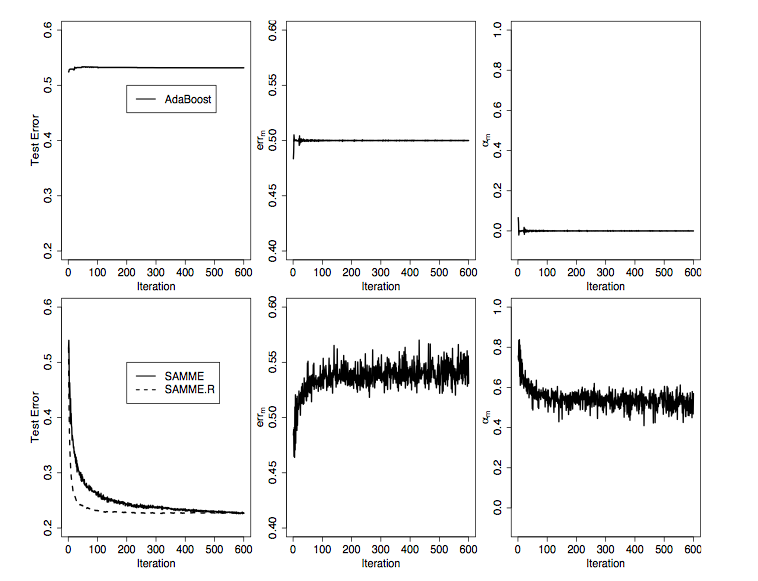
\includegraphics[width=1.0\textwidth]{confronto_samme_m2.png}}%
 \caption{Confronto grafico fra Adaboost (prima riga) 
e SAMME (seconda riga) su una semplice simulazione a tre classi. La taglia di 
training \`e 3000, mentre la taglia di test \`e 10000. Sono stati utilizzati come classificatori weak dieci 
alberi di decisione.}
 \label{fig:key}
\end{figure}

Come \`e gi\`a stato detto, Adaboost si arresta dopo che l'errore supera 1/2. Questo non riguarda SAMME: 
anche se l'errore diventasse maggiore (o uguale) a 1/2, il 
valore \begin{math}\alpha \end{math} sarebbe ancora positivo; 
da ci\`o, gli esempi di training classificati in maniera errata prendono pi\`u peso, 
e l'errore di test si mantiene 
decrescente anche dopo 600 iterazioni. \\
\newline
\subsection{Giustificazione teorica}
Come accennato in precedenza la costante additiva 
\begin{math}\log(K-1)\end{math} in (\ref{eq:alg}) non 
\`e artificale, crea un filtro equivalente a fittare un modello addittivo 
attraverso la forward stagewise. Friedman svilupp\`o una prospettiva statistica sull'originale algoritmo adaboost 
a due classi, che induce a vedere l'adaboost a due classi come un modello addittivo 
forward stagewise attraverso la funzione loss esponenziale:
\begin{center}
\begin{math} L(y,f) = e^{-yf(\textbf{x})} \end{math}
\end{center}
dove \begin{math}y=(\mathbbm{1}(y = 1) - \mathbbm{1}(y = 2))\in \left\{-1,1\right\}\end{math} 
in un ambiente di classificazione a due classi. Non \`e difficile mostrare che l'argmin 
della funzione loss esponenziale \`e la met\`a della trasformazione logit: 
\begin{center}
 \begin{math} f^*(\textbf{x})=\underset{f(\textbf{x})}{\operatorname{argmin}}L(y,f)= 
\frac{1}{2}\end{math}
           \begin{math}\frac{(Prob (y) =1|\textbf{x})}{(Prob (y)=2|\textbf{x})}\end{math}
\end{center}
La regola di classificazione ottimale di Bayes concorda col segno di \begin{math}f^*(x)\end{math}, ovvero
\begin{center}
 \begin{math}
 \underset{y}{\operatorname{argmax}} 
 \end{math} Prob\begin{math}
                 (Y=y | \textbf{X=x}) =
                \end{math} sign\begin{math}
                                (f^*(\textbf{x}))
                               \end{math}



\end{center}

\subsection{Nuova loss function multiclasse}
In un ambiente di classificazione multiclasse, si pu\`o ricodificare l'output \begin{it}y\end{it} 
con un vettore \textbf{y} \begin{it}K\end{it}-dimensionale, 
dove tutte le entrate sono uguali a \begin{math}-\frac{1}{K-1} \end{math}
 eccetto a 1 in posizione \begin{it}k \end{it} se \begin{it}c=k\end{it}, 
cio\`e \begin{math} \textbf{y} =(y_1,...,y_K)^t\end{math} e:
\begin{center}
 \begin{equation}\label{eq:vet_mc}
 y_k=\begin{cases}1 & y=k\\
-\frac{1}{K-1} & y\ne k\end{cases}
\end{equation}
\end{center}
La stessa architettura \`e stata utilizzata in altri ambienti come ad esempio nella versione multiclasse di 
support vector machine (SVM).\\
\newline
La generalizzazione della funzione loss esponenziale al caso multivariato segue naturalmente:
 \begin{center}
 \begin{equation} \label{eq:loss_mc}
L(\textbf{y,f}) =
exp(-\frac{1}{K}(y_1f_1 + ... + y_Kf_K)) = (-\frac{1}{K}\begin{bf}y^tf\end{bf})
\end{equation}
\end{center}
dove \begin{math}f_k\end{math} corrisponde alla classe \begin{it}k\end{it}.\\
\newline
Si noti che c'\`e bisogno di alcuni vincoli su \begin{bf}f\end{bf} affinch\`e (\ref{eq:loss_mc}) 
sia stimabile, d'altra parte, 
aggiungendo qualsiasi costante a tutto \begin{math}f_k\end{math} non cambia la perdita (loss). Viene scelto di usare il 
vincolo di simmetria:
\begin{center}
 \begin{math} f_1 + ... + f_K = 0
\end{math}
\end{center}
In questo modo, quando K=2 la funzione loss esponenziale multinomiale si riduce alla funzione loss esponenziale 
classica biclasse.\\
\newline
In maniera simile al caso a due classi, si \`e interessati a scoprire cosa questa funzione loss esponenziale 
multiclasse stimi. A questo si pu\`o rispondere cercando il suo argmin. 
In particolare, si \`e interessati a:
\begin{center}
 \begin{math} \underset{\begin{bf}f(x)\end{bf}}{\operatorname{argmin}}\end{math} 
E\begin{math}_{\begin{bf}Y|x\end{bf}} \end{math}exp
\begin{math}(-\frac{1}{K}(Y_1f_1 + ... + Y_Kf_K))
\end{math}
\end{center}
\begin{center}
 soggetto al vincolo \begin{math}f_1 + ... + f_K = 0
\end{math}
\end{center}
Segue dai calcoli:
\begin{center}
\begin{math}
exp (-\frac{1}{K}( f_1(\textbf{x}) - \frac{f_2(\textbf{x})}{K-1} - \dots - \frac{f_K(\textbf{x})}{K-1}) Prob ((y)=1|\textbf{x}) + 
\dots  
\end{math}
\end{center}

\begin{center}
 \begin{math}
  + exp (-\frac{1}{K}( \frac{f_1(\textbf{x})}{K-1} - \frac{f_2(\textbf{x})}{K-1} - \dots - f_K(\textbf{x}) 
Prob ((y)=K|\textbf{x}) =
 \end{math}
\end{center}

\begin{center}
 \begin{math}
  exp(-\frac{1}{K}(F_1(\textbf{x}) + \frac{f_1(\textbf{x})}{K-1})) Prob ((y)=K|\textbf{x})
 \end{math}

\end{center}


\begin{center}
 \begin{math}
  + exp(-\frac{1}{K}(f_K(\textbf{x}) + \frac{f_K(\textbf{x})}{K-1})) Prob ((y)=K|\textbf{x})
 \end{math}

\end{center}


Attraverso il metodo dei moltiplicatori di Lagrange questo problema di ottimizzazione vincolata pu\`o 
esser riscritto come:
\begin{center}
 \begin{math}
  exp (-\frac{f_1(\textbf{x})}{K-1} Prob((y)=1|\textbf{x})) + \dots 
+ exp (-\frac{f_K(\textbf{x})}{K-1} Prob((y)=K|\textbf{x})) + 
 \end{math}
\end{center}
\begin{center}
 \begin{math}
-  \lambda (f_1(\textbf{x}) + \dots + f_K(\textbf{x})
 \end{math}

\end{center}
dove \begin{math}
      \lambda 
     \end{math}  \`e il moltiplicatore di Lagrange. Calcolando le derivate rispetto a 
\begin{math}
 f_k
\end{math} e \begin{math}
              \lambda
             \end{math}, troviamo:
\begin{center}
 \begin{math}
  -\frac{1}{K-1} exp (-\frac{f_1(\textbf{x})}{K-1} Prob((y)=1|\textbf{x}) -\lambda = 0
 \end{math}

\end{center}
\begin{center}
 \begin{math}
 \vdots
\end{math}
\end{center}

\begin{center}
 \begin{math}
  -\frac{1}{K-1} exp (-\frac{f_K(\textbf{x})}{K-1} Prob((y)=K|\textbf{x}) -\lambda = 0
 \end{math}
\end{center}
\begin{center}
 \begin{math}
  f_1 + ... + f_K = 0
 \end{math}

\end{center}

Risolvendo questo sistema di equazioni, si ottiene:
\begin{center}
 \begin{equation}\label{eq:lagrange}
 f_k^*(\textbf{x}) = (K-1) (log Prob(c=k|\textbf{x}) - \frac{1}{K}\sum_{k'=1}^K log Prob(y=k'|\textbf{x}))
\end{equation}
\end{center}
con k=1,...,K; perci\`o:
\begin{center}
 \begin{math} \underset{k}{\operatorname{argmax}} f_k^*(\textbf{x}) = 
\underset{k}{\operatorname{argmax}}Prob(c=k|\textbf{x})
\end{math}
\end{center}
che \`e la regola di classificazione ottimale di Bayes per l'errore. Questo giustifica l'uso della 
funzione loss esponenziale multiclasse. L'equazione (\ref{eq:lagrange}) trova anche un modo per recuperare 
\begin{math}
 Prob( y = k | \textbf{x})
\end{math} una volta che \begin{math}
                          f^*_k(\textbf{x})
                         \end{math} sono stimate:
\begin{center}
 \begin{math}
  Prob( c = k | \textbf{x}) = \frac{exp(\frac{1}{K-1}f^*_k(\textbf{x}))}{exp(\frac{1}{K-1}f^*_1(\textbf{x}))+ ... + 
exp(\frac{1}{K-1}f^*_k(\textbf{x}))}
 \end{math}
 per k =1, ..., K
\end{center}


\subsection{SAMME e FSAM}
Adesso si mostrer\`a che l'algoritmo SAMME \`e equivalente al modello addittivo per forward stagewise utilizzando 
la loss function esponenziale multiclasse trovata nel paragrafo precedente (\ref{eq:loss_mc}). Inizialmente si lavorer\`a con la loss function 
canonica, successivamente verr\`a applicata quella multiclasse.\\
\newline
Avendo dei dati di training, ci auguriamo di trovare \begin{math}f(\textbf{x}) = 
(f_1(\textbf{x})+ ...+ f_K(\textbf{x}))^t \end{math} tale che:
\begin{center}
 \begin{equation}\label{eq:minimo}
 \underset{f(\textbf{x})}{\operatorname{min}} \sum_{i=i}^mL(\textbf{y}_i,f(\textbf{x}_i))
\end{equation}
\end{center}

 soggetto al vincolo
\begin{center} 
\begin{equation}\label{eq:vincolo}
f_1(\textbf{x}) + ... + f_K(\textbf{x}) = 0
\end{equation}
\end{center}
Si consideri \begin{math}
              f(\textbf{x})
             \end{math} che ha la seguente forma:
\begin{center}
 \begin{math} f(\textbf{x}) = \sum_{t=1}^T\beta_t g_t(\textbf{x})
\end{math}
\end{center}
dove \begin{math}
      \beta_t \in \mathbb{R}
     \end{math} sono coefficienti e \begin{math}
                                    g_t(\textbf{x})
                                   \end{math} sono funzioni base. Ordiniamo a \begin{math}
                                    g_t(\textbf{x})
                                   \end{math} 
di soddisfare il vincolo \begin{math}g_1(\textbf{x}) + ... + g_K(\textbf{x}) = 0
\end{math}.\\
\newline 
Per esempio,la funzione \begin{math}
                                    g_t(\textbf{x})
                                   \end{math} che si considera prende valore in uno dei K possibili vettori 
K-dimensionali; precisamente, dato \begin{math}\textbf{x}\end{math}, 
\begin{math}\textbf{g(x)}\end{math} mappa \begin{math}\textbf{x}\end{math} su \begin{math}
                                                                               \mathcal{Y}
                                                                              \end{math}
\begin{center}
 \begin{math}
  g: \textbf{x} \in \mathbb{R}^p \rightarrow \mathcal{Y}
 \end{math}

\end{center}
dove \begin{math}
      \mathcal{Y}
     \end{math} contiene K vettori K-dimensionali.




Il modello forward stagewise approssima la soluzione delle richieste (\ref{eq:minimo})-
(\ref{eq:vincolo}) sequenzialmente 
aggiungendo nuove funzioni base all'espansione senza adattare i parametri e coefficienti di quelli che erano 
gi\`a stati aggiunti. Specificatamente, l'algoritmo parte con \begin{math}
                                                               f_0(\textbf{x}) = 0
                                                              \end{math} sequenzialmente seleziona nuove 
funzioni base da un dizionario e le aggiunge:
\begin{itemize}
 \item Inizializza \begin{math}f_0(x) = 0 \end{math}
\item Per \begin{math}t = 1 ... T \end{math} iterazioni\\
\newline
Calcola:
\begin{center}
 \begin{math} (\beta_t,g_t(\textbf{x})) = \underset{\beta,g}{\operatorname{min}}
\sum_{i=1}^m L(\textbf{y}_i, f_{t-1}(\textbf{x}_i) + \beta g(\textbf{x}_i))
\end{math}
\end{center}
Assegna:
\begin{center}
 \begin{math} f_t(\textbf{x}) = f_{(t-1)}(\textbf{x}) + \beta_t g_t(\textbf{x})
\end{math}
\end{center}
\end{itemize}
Il passo cruciale di questo studio avviene al calcolo di  \begin{math} (\beta_t,g_t)
\end{math}, infatti, usando la funzione loss esponenziale multivariata:
\begin{center}
 \begin{equation} \label{eq:sol1}
(\beta_t,g_t) = \underset{\beta,g}{\operatorname{argmin}} \sum_{i=i}^m exp(
-\frac{1}{K}\textbf{y}_i^t(f_{t-1}(\textbf{x}_i) + \beta g(\textbf{x}_i))\end{equation}
\end{center}
\begin{center}
 \begin{equation}\label{eq:sol2}
= \underset{\beta,g}{\operatorname{argmin}} \sum_{i=1}^m D_t(i) exp(
 -\frac{1}{K}\beta \textbf{y}_i^tg(\textbf{x}_i))
\end{equation}                                                                      
\end{center}
dove \begin{math}D_t(i) =\end{math} exp \begin{math}-\frac{1}{K}\textbf{x}_i^t(f_{t-1}(\textbf{x}_i)\end{math} sono i pesi non 
normalizzati.\\
\newline
Si noti che ogni funzione \begin{math}
                           g(\textbf{x})
                          \end{math} nei K vettori K-dimensionali ha una corrispondenza con un classificatore 
multiclasse \begin{math}
             h(x)
            \end{math}
 come segue:
\begin{center}
 \begin{equation}\label{eq:cor1}
  h(x) = k, 
 \end{equation}
se \begin{math} g_k(\textbf{x})=1\end{math}
                                 
\end{center}
e vice versa.

Quindi, risolvere \begin{math}g_t(\textbf{x})\end{math} \`e equivalente a trovare il classificatore multi-classe 
\begin{math}h_t(x)\end{math} che pu\`o generare \begin{math}g_t(\textbf{x})\end{math}. Di seguito si proceder\`a 
quindi con lo svolgimento della soluzione:
\begin{center}
\begin{equation}\label{eq:T_m}
 h_t (\textbf{x})= argmin  \sum_{i=1}^m D_t(i) \mathbbm{1}(y_i\ne h(\textbf{x}_i))
\end{equation}                                                                      
\end{center}
\begin{center}
\begin{equation}\label{eq:beta_m}
\beta_t = \frac{(K-1)^2}{K} ( log \frac{1-\varepsilon_t}{\varepsilon_t} + log(K-1)
\end{equation}                                                                      
\end{center}
Dove \begin{math}\varepsilon_t\end{math} \`e definito come :
\begin{center}
\begin{math}
 \varepsilon_t = \sum_{i=1}^m D_t(i) \mathbbm{1}(c_i\ne h(\textbf{x}_i))/\sum_{i=1}^m D_t(i)
\end{math}                                                                      
\end{center}
Adesso, per ogni valore fissato \begin{math}
                                 \beta >0
                                \end{math}, utilizzando la definizione (\ref{eq:cor1})
 
si pu\`o esprimere il criterio in (\ref{eq:sol2}) come:

\begin{center}
\begin{math}
 \sum_{y_i=h(x_i)}D_t(i)\end{math}exp
\begin{math}(-\frac{\beta}{K-1} - \sum_{y_i\ne h(x_i)}D_t(i)\end{math}exp
\begin{math}(\frac{\beta}{(K-1)^2})=
\end{math}                                                                      
\end{center}
\begin{center}
\begin{equation}\label{eq:sol3}
 exp(-\frac{\beta}{K-1}\sum_i D_t(i) + (exp
(\frac{\beta}{(K-1)^2}) - exp
(\frac{\beta}{K-1}))\sum_i^m D_t(i)
\end{equation}                                                                      
\end{center}
Solo l'ultima somma dipende dal classificatore \begin{math}h(\textbf{x})\end{math}, 
noi prendiamo quella che contiene la (\ref{eq:T_m}). 
A questo punto, inserendo (\ref{eq:T_m}) in (\ref{eq:sol2}) e risolvendo per \begin{math}
                                 \beta
                                \end{math}, si ottiene (\ref{eq:beta_m}).\\
\newline
Il modello viene poi aggiornato:
\begin{center}
\begin{math}
 f_t(\textbf{x}) = f_{t-1}(\textbf{x}) + \beta_t g_t(\textbf{x})
\end{math}                                                                      
\end{center}
e i pesi per la prossima iterazione saranno:
\begin{center}
\begin{math}
 D_t(i) \leftarrow D_t(i)\end{math} exp
 \begin{math}(-\frac{1}{K}\beta_t y_i^tg_t(\textbf{x}_i)) \end{math}                                                                   
\end{center}
Questo equivale a:
\begin{center}
\begin{equation}\label{eq:finale}
 D_t(i) exp(-\frac{(K-1)^2}{K^2} \alpha_t y_i^t g_t(\textbf{x}_i) )
= \begin{cases}D_t(i) exp(-\frac{(K-1)^2}{K} \alpha_t) & y_i=h(x_i)\\
  D_t(i) exp(\frac{1}{K}\alpha_t) & y_i\ne h(x_i) 
  \end{cases}
\end{equation}                                                                      
\end{center}
Dove \begin{math}\alpha_t \end{math} \`e definita in (\ref{eq:alg}) col termine extra log(K-1), e il nuovo peso 
\`e equivalente al peso dell'algoritmo SAMME aggiornato dopo la normalizzazione.




\section{Adaboost.MH}
Adaboost.MH \`e una generalizzazione del filtro M2. Potendo la singola osservazione x appartenere a diverse 
etichette (concetto multi-label), 
si introduce un nuovo algoritmo che, con diversi concetti di funzione loss, affronta la possibilit\`a 
di cambiamento delle label. Si 
noti, come si mostrer\`a in questo paragrafo, che nel caso ogni osservazione appartenga a una sola classe, questo 
filtro si riduce ad Adaboost.M2.\\
\newline
Sia \begin{math}
     Y 
    \end{math} un set finito di etichette, e sia \begin{math}
                                                           k = |Y|
                                                          \end{math}. In un ambiente di classificazione 
tradizionale, ogni esempio \begin{math}
     x \in X 
    \end{math} alla singola classe \begin{math}
     y \in Y 
    \end{math}, quindi gli esempi etichettati sono coppie \begin{math}
                                                           (x,y)
                                                          \end{math}. Lo scopo poi, generalmente, 
\`e di trovare un'ipotesi \begin{math}
                         H : X \rightarrow Y
                        \end{math} che minimizza la probabilit\`a che \begin{math}
                                                                       y \ne H(x)
                                                                      \end{math} su un nuovo 
esempio osservato \begin{math}  (x,y) \end{math}. \\
\newline
Nel caso multi-label, ogni istanza \begin{math}
     x \in X 
    \end{math} pu\`o appartenere a diverse classi in \begin{math}
                                                      Y
                                                     \end{math}. Quindi, un esempio etichettato \`e una coppia 
\begin{math}(x,\mathcal{Y})\end{math} dove \begin{math}
                                  \mathcal{Y} \subseteq Y
                                 \end{math} nel set di etichette assegnate a x. Il caso single-label \`e 
chiaramente un caso speciale quando \begin{math} |Y| = 1   \end{math} per tutte le osservazioni.\\
Non \`e chiaro in questo ambiente precisamente come formalizzare lo scopo dell'algoritmo di apprendimento, e, in 
generale, la ``giusta'' formalizzazione pu\`o dipendere dal problema. Una possibilit\`a \`e di cercare un'ipotesi 
che prova a predire solo una delle etichette assegnate a un esempio. In altre parole, lo scopo \`e di trovare 
\begin{math} H : X \rightarrow Y\end{math} che minimizza la probabilit\`a che 
\begin{math}
 H(x) \notin \mathcal{Y}
\end{math} su una nuova osservazione \begin{math}
                                      (x,\mathcal{Y})
                                     \end{math}. Chiamiamo questa misura ``un errore'' delle ipotesi 
\begin{it}H\end{it} siccome misura la probabilit\`a di non ottenere anche una tra le etichette corrette. 
Si denota ``un errore'' di un'ipotesi \begin{it}h\end{it} rispetto alla distribuzione \begin{it}D\end{it} 
sulle osservazioni \begin{math}(x,\mathcal{Y})\end{math} in questo modo:
\begin{center}one-err
 \begin{math}
  _D(H) = Pr_{(x,Y) \texttildelow D}\left[H(x) \notin \mathcal{Y}\right]
 \end{math}

\end{center}
Si noti che, per un problema di classificazione single-label, ``un errore'' \`e il corrispondente dell'errore 
ordinario. Nel paragrafo seguente, si introdurr\`a una nuova misura di perdita (loss) che pu\`o essere utilizzata 
in questo ambiente multiclasse, chiamata Hamming loss (o ranking loss). Si analizzeranno inoltre le modifiche 
appropriate all'Adaboost per via di questo nuovo concetto di perdita (loss).

\subsection{Utilizzo della Hamming loss per i problemi multi-classe}
Si supponga adesso che lo scopo sia di predire tutte e solo le etichette corrette. Ovvero, l'algoritmo 
di apprendimento genera un'ipotesi che predice sets di etichette, e la loss dipende su come queste predizioni 
differiscono da una che \`e stata osservata. Perci\`o, 
\begin{math} H : X \rightarrow 2^Y\end{math} e, rispetto alla distribuzione \begin{it} D\end{it} 
la loss \`e:
\begin{center}
 \begin{math}
 \frac{1}{k} E_{(x,Y) \texttildelow  D} \left[|h(x) \mathcal{4} \mathcal{Y} | \right]
 \end{math}
\end{center}
dove \begin{math}
      \mathcal{4}
     \end{math} denota la differenza simmetrica (il valore 1/k \`e utilizzato solo per assicurarsi che 
il valore stia in \begin{math}
                   \left[0,1\right]
                  \end{math}). Chiamiamo questa misura \begin{it}
                                                        Hamming loss
                                                       \end{it} di H, e la denotiamo come
\begin{math}
 hloss_D(H)
\end{math}. Per minimizzare la Hamming loss, si pu\`o, in maniera naturale, decomporre il problema in 
\begin{it}k\end{it} problemi di classificazione binaria ortogonali. Si pensa a 
\begin{math}\mathcal{Y}\end{math} come \begin{it}k\end{it} 
etichette binarie (dipendendo da che un'etichetta \begin{it}y\end{it} sia o 
non sia inclusa in \begin{math}\mathcal{Y}\end{math}). 
Similmente, \begin{it}h(x)\end{it} pu\`o essere vista come \begin{it}k\end{it} predizioni binarie. 
La Hamming loss poi pu\`o essere considerata come una media dell'errore di \begin{it}h\end{it} su questi 
\begin{it}k\end{it} problemi binari. \\
Per  \begin{math} \mathcal{Y} \subseteq Y \end{math}, si definisce \begin{math}
                                                                    \mathcal{Y}\left[l\right]
                                                                   \end{math} per \begin{math}
                                                                                   l \in Y
                                                                                  \end{math} essere:
\begin{center}
 \begin{math}
   \mathcal{Y}\left[l\right] = \begin{cases}1 & l \in \mathcal{Y}\\
-1 & l\notin \mathcal{Y}\end{cases}
 \end{math}

\end{center}
Per semplificare la notazione, si identifica anche qualsiasi funzione 
\begin{math} H : X \rightarrow 2^Y\end{math} con una corrispondente funzione a due 
argomenti \begin{math}
           H : X \times Y \rightarrow \left\{-1,1\right\}
          \end{math} definita da \begin{math}
                                  H(x,l) = H(x)\left[l\right]
                                 \end{math}\\
\newline
Con la riduzione alla classificazione binaria in mente, \`e piuttosto inequivocabile vedere come utilizzare 
il boosting per minimizzare la Hamming loss. L'idea principale della riduzione \`e semplicemente ripetere ogni 
esempio di training \begin{math}
                     (x_i,Y_i)
                    \end{math} per \begin{it}k\end{it} esempi 
\begin{math}
 ((x_i,l),Y_i\left[l\right])
\end{math} per \begin{math}
                l \in \mathcal{Y}
               \end{math}. Il risultato \`e un algoritmo di boosting chiamato proprio Adaboost.MH che mantiene 
una distribuzione sugli esempi \begin{it}i\end{it} e etichette \begin{it}l\end{it}.\\
Come per ogni classificatore, si riporta un breve schema con i passaggi essenziali dell'algoritmo.
\begin{itemize}
 \item Dati: \begin{math}
              (x_1,Y_1), ..., (x_m,Y_m)
             \end{math} dove \begin{math}
                              x_i \in X, \mathcal{Y}_i \subseteq Y
                             \end{math}
 \item Si inizializza \begin{math}
                       D_1(i,l) = 1/(mk)
                      \end{math}
 \item Per t = 1, ..., T
\end{itemize}

\begin{enumerate}
 \item Viene chiamato il weak learner utilizzando la distribuzione \begin{math}
                                                             D_t
                                                            \end{math}
 \item Il weak learner, in risposta, genera un'ipotesi \begin{math}
                               h_t : X \times Y \rightarrow \mathbb{R}
                              \end{math}
 \item Viene calcolato \begin{math}
                \alpha_t \in \mathbb{R}
               \end{math}
 \item Viene aggiornata:

\end{enumerate}
\begin{center}
 \begin{math}
  D_{t+1}(i,l) = \frac{D_t(i,l)exp(-\alpha_t Y_i\left[l\right] h_t (x_i,l))}{Z_t}
 \end{math}
\end{center}
Dove \begin{math}
      Z_t
     \end{math} \`e un fattore di normalizzazione (scelto in modo tale che 
\begin{math}
 D_{t+1}
\end{math} sia una distribuzione).\\
L'output sar\`a:
\begin{center}
 \begin{math}
  H(x,l) = sign ( \sum_{t=1}^T \alpha_t h_t (x,l))
 \end{math}

\end{center}
Al passo \begin{it}t\end{it}, il weak learner accetta cos\`i una distribuzione \begin{math}
                                                                               D_t
                                                                              \end{math} (in aggiunta al 
training set), e genera un'ipotesi weak \begin{math}
                                         h_t :X \times Y \rightarrow \mathbb{R}
                                        \end{math}. Questa riduzione conduce anche alla scelta dell'ipotesi finale 
mostrata nello schema. \\
\newline
\textbf{Teorema 3.} Assumendo la notazione dello schema appena esposto, il seguente margine superiore per la 
Hamming loss di H sui dati di training:
\begin{center}hloss(H)
 \begin{math}
  \le \prod_{t=1}^T Z_t
 \end{math}
\end{center}
Si pu\`o ora applicare l'idea della sezione precedente in questo problema di classificazione binaria. Come prima, 
lo scopo \`e minimizzare:
\begin{center}
 \begin{math}
  Z_t = \sum{i,l} D_t(i,l)exp(-\alpha_t \mathcal{Y}_i\left[l\right] h_t (x_i,l))
 \end{math}

\end{center}
per ogni iterazione.\\
\newline
Se si richiede che ad ogni passo \begin{math} h_t  \end{math} abbia range in \begin{math}                                                                                                                                                  
\left[-1,+1\right]\end{math}, 
poi bisognerebbe scegliere 
 \begin{center}
 \begin{math}
  \alpha_t = \frac{1}{2}
 \end{math}ln\begin{math}
              (\frac{1+r_t}{1-r_t})
             \end{math}
\end{center} 
dove:
\begin{center}
 \begin{math}
  r_t = \sum_{i,l} D_t(i,l) \mathcal{Y}_i\left[l\right] h_t (x_i,l)
 \end{math}
\end{center}
Questo porta a:
\begin{center}
 \begin{math}
  Z_t = \sqrt{1-r_t^2}
 \end{math}
\end{center}
E lo scopo del weak learner diventa la minimizzazione di \begin{math}
                                                          |r_t|
                                                         \end{math}.\\
Si noti che (1-\begin{math}
                r_t
               \end{math})/2 equivale a:
\begin{center}
 \begin{math}
  Pr_{(i,l)\texttildelow D}\left[h_t(x_i,l) \ne \mathcal{Y}_i\left[l\right]\right]
 \end{math}

\end{center}
Facciamo un esempio di come minimizzare \begin{math}
                                                          |r_t|
                                                         \end{math}. Si supponga che lo scopo sia di trovare 
un'ipotesi weak \begin{math}
                            h_t
                           \end{math} che ``ignora'' l'istanza \begin{it}x\end{it}
 e predice soltanto sulla base dell'etichetta \begin{it}l\end{it}. Si pu\`o quindi omettere l'argomento \begin{it}x\end{it}
 e scrivere \begin{math}
                                                             h_t(x,l) = h_t(l)
                                                            \end{math}; oltre che al pedice\begin{it}
                                                                                             t
                                                                                            \end{it}. 
Per simmetria, minimizzare -\begin{it}r\end{it} equivale a massimizzare \begin{it}r\end{it}. Perci\`o, bisogna 
solo trovare \begin{it}h\end{it} che massimizzi 
\begin{center}
 \begin{math}
  r = \sum_{i,l} D_t(i,l) \mathcal{Y}_i\left[l\right] h_t (l)
 \end{math}
\end{center}
  \begin{center}
 \begin{math}
  = \sum_l 
 \end{math} sign\begin{math}
                 \sum_i D(i,l) \mathcal{Y}_i\left[l\right]
                \end{math}

\end{center}



 
 












 














                 
 













   


   
  
 




\ \
